% SCUDEM preliminary round: Euler and RK4 (Beamer, 16:9)
% Workflow: 1) run scudem_euler_rk4.m in MATLAB  2) compile with
%   latexmk -pdf presentation.tex     (or run pdflatex twice)
\documentclass[aspectratio=169,11pt]{beamer}

\usepackage[T1]{fontenc}
\usepackage{lmodern}
\usepackage{amsmath,amssymb}
\usepackage{booktabs}
\usepackage{graphicx}
\usepackage{listings}
\usepackage{tikz}
\usetikzlibrary{arrows.meta,decorations.pathreplacing,calc}

%% ---------- Palette ----------
\definecolor{navy}{HTML}{14284B}
\definecolor{accent}{HTML}{D9483B}
\definecolor{euler}{HTML}{D93A26}
\definecolor{rk}{HTML}{1A5AB8}
\definecolor{soft}{HTML}{EEF2F8}
\definecolor{mid}{HTML}{5B6B85}

%% ---------- Theme ----------
\usetheme{default}
\usefonttheme{professionalfonts}
\setbeamertemplate{navigation symbols}{}
\setbeamersize{text margin left=1.2cm,text margin right=1.2cm}
\setbeamercolor{normal text}{fg=navy}
\setbeamercolor{structure}{fg=rk}
\setbeamercolor{block title}{bg=soft,fg=navy}
\setbeamercolor{block body}{bg=soft,fg=navy}
\setbeamerfont{block title}{series=\bfseries,size=\normalsize}
\setbeamertemplate{blocks}[rounded][shadow=false]
\setbeamerfont{frametitle}{size=\Large,series=\bfseries}
\setbeamertemplate{frametitle}{%
  \vskip 2.2ex
  {\usebeamerfont{frametitle}\color{navy}\insertframetitle}\par
  \vskip 0.8ex
  {\color{accent}\rule{2cm}{2.4pt}}\par
}
% Footer: fixed-width box, so the slide number always stays inside the
% right margin (the \hspace* margins cannot be discarded by TeX).
\setbeamertemplate{footline}{%
  \hbox to \paperwidth{%
    \hspace*{1.2cm}%
    {\fontsize{7}{8}\selectfont\color{mid}SCUDEM Preliminary Round \quad|\quad Euler and Runge--Kutta 4}%
    \hfill
    {\fontsize{7}{8}\selectfont\color{mid}\insertframenumber\,/\,\inserttotalframenumber}%
    \hspace*{1.2cm}}%
  \vskip 0.45cm}
\setbeamertemplate{itemize item}{\color{accent}\tiny$\blacksquare$}
\setbeamertemplate{itemize subitem}{\color{accent}\tiny$\blacktriangleright$}

%% ---------- Helpers ----------
% Include a MATLAB figure if it exists, otherwise show a placeholder box.
\newcommand{\safefig}[2][\linewidth]{%
  \IfFileExists{figs/#2.png}%
    {\includegraphics[width=#1]{figs/#2.png}}%
    {\fbox{\parbox{\dimexpr#1-2\fboxsep-2\fboxrule\relax}{\centering\vspace{3em}Run \texttt{scudem\_euler\_rk4.m} to create \texttt{figs/\detokenize{#2}.png}\vspace{3em}}}}}

\newcommand{\eul}[1]{{\color{euler}#1}}
\newcommand{\rkc}[1]{{\color{rk}#1}}

% numbered agenda badge (used on the Outline slide)
\newcommand{\agn}[1]{\tikz[baseline=(n.base)]\node[circle,fill=accent,text=white,
  inner sep=2.6pt,minimum size=0.62cm,font=\small\bfseries] (n) {#1};}

\lstdefinestyle{mat}{
  language=Matlab, basicstyle=\ttfamily\footnotesize, keywordstyle=\color{rk}\bfseries,
  commentstyle=\color{mid}\itshape, stringstyle=\color{accent},
  backgroundcolor=\color{soft}, frame=none, xleftmargin=6pt, xrightmargin=6pt,
  aboveskip=0pt, belowskip=0pt, columns=fullflexible, keepspaces=true, showstringspaces=false}

\title{Modelling with First-Order ODEs}
\subtitle{Euler's Method and Runge--Kutta 4 in MATLAB}
\author{Rahul Sanklecha}   % edit: add team members / institution
\date{}

\begin{document}

%% ================= 1. Title =================
\begin{frame}[plain]
  \begin{tikzpicture}[remember picture,overlay]
    \fill[navy] (current page.south west) rectangle (current page.north east);
    \fill[accent] ([xshift=1.2cm,yshift=-0.3cm]current page.north west) rectangle ++(2.2cm,0.09cm);
    % decorative slope-field motif
    \foreach \i in {0,...,9}{\foreach \j in {0,...,4}{
      \pgfmathsetmacro{\s}{0.5*(\i/9)*(1-\i/9)*4}
      \draw[white,opacity=0.10,line width=1.2pt]
        ([xshift={9.2cm+\i*0.42cm},yshift={0.9cm+\j*0.62cm}]current page.south west)
        -- ++({0.28},{0.28*\s});}}
  \end{tikzpicture}
  \vfill
  {\color{white}\fontsize{28}{32}\selectfont\bfseries Modelling with\\First-Order ODEs\par}
  \vskip 1.2ex
  {\color{white!75!navy}\fontsize{15}{18}\selectfont Euler's method and Runge--Kutta 4 in MATLAB\par}
  \vskip 4ex
  {\color{white}\large Rahul Sanklecha\par}
  {\color{white}\large Rishil Chudasama\par}
  {\color{white}\large Shashwat Saxena\par}
  \vskip 1.5ex
  {\color{white!60!navy}\small SCUDEM Preliminary Round\par}
  \vfill
\end{frame}

%% ================= 2. Outline =================
\begin{frame}{Outline}
  \renewcommand{\arraystretch}{1.75}
  \begin{tabular}{@{}c@{\hspace{1em}}l@{\hspace{1.6em}}l@{}}
    \agn{1} & \textbf{The Problem}          & {\small\color{mid}Why we need numerical methods; slope fields}\\
    \agn{2} & \textbf{Our Model}            & {\small\color{mid}Logistic growth and its exact solution}\\
    \agn{3} & \textbf{The Two Methods}      & {\small\color{mid}\eul{Euler} and \rkc{RK4}, plus one worked step}\\
    \agn{4} & \textbf{MATLAB Implementation}& {\small\color{mid}The two update loops}\\
    \agn{5} & \textbf{Results}              & {\small\color{mid}Curves, error measurement, convergence, table}\\
    \agn{6} & \textbf{Cost and Conclusions} & {\small\color{mid}Accuracy per evaluation of $f$}\\
  \end{tabular}
\end{frame}

%% ================= 3. Problem =================
\begin{frame}{The problem: most ODEs cannot be solved exactly}
  \begin{center}
    \Large $\displaystyle \frac{dy}{dt} = f(t,y), \qquad y(t_0)=y_0$
  \end{center}
  \vspace{1.2ex}
  \begin{columns}[T]
    \column{0.31\textwidth}
    \begin{block}{Reality}
      Nonlinear models rarely have a closed-form solution.
    \end{block}
    \column{0.31\textwidth}
    \begin{block}{Idea}
      Use the slope $f(t,y)$ to walk forward in small steps of size $h$.
    \end{block}
    \column{0.31\textwidth}
    \begin{block}{This talk}
      \eul{Euler}: one slope per step.\\ \rkc{RK4}: four slopes per step.
    \end{block}
  \end{columns}
\end{frame}

%% ================= 4. Slope field =================
\begin{frame}{The slope field: the ODE as a map of arrows}
  \begin{columns}[c]
    \column{0.62\textwidth}
    \safefig{fig_slopefield}
    \column{0.34\textwidth}
    Every point $(t,y)$ carries a slope $f(t,y)$.\\[1.5ex]
    A solution is a curve that follows the arrows.\\[1.5ex]
    A numerical method \textbf{follows the arrows in discrete steps}.
  \end{columns}
\end{frame}

%% ================= 5. Model =================
\begin{frame}{Our model: logistic population growth}
  \begin{columns}[c]
    \column{0.45\textwidth}
    \[
      \frac{dP}{dt} = rP\Bigl(1-\frac{P}{K}\Bigr)
    \]
    \vspace{-1ex}
    \begin{itemize}
      \item $r=0.5$ \; growth rate
      \item $K=100$ \; carrying capacity
      \item $P(0)=10$
    \end{itemize}
    \vspace{1ex}
    \begin{block}{Exact solution (our benchmark)}
      \[ P(t)=\frac{K}{1+\frac{K-P_0}{P_0}e^{-rt}} \]
    \end{block}
    \column{0.5\textwidth}
    \safefig{fig_growthrate}
  \end{columns}
\end{frame}

%% ================= 6. Euler =================
\begin{frame}{Euler's method: follow the tangent}
  \begin{columns}[c]
    \column{0.60\textwidth}
    \begin{center}
    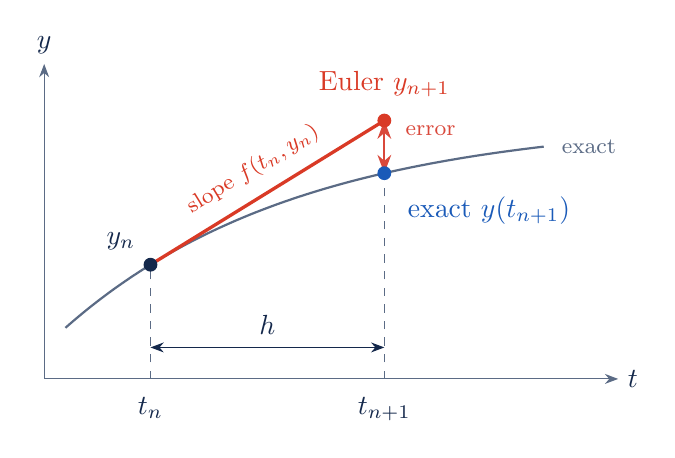
\begin{tikzpicture}[x=1.35cm,y=1.0cm,>=Stealth]
      % model: y' = 0.45(3.3-y),  exact y = 3.3 - 2.9 e^{-0.45 t}
      \pgfmathsetmacro{\tStart}{1.0}
      \pgfmathsetmacro{\hStep}{2.2}
      \pgfmathsetmacro{\tNext}{\tStart+\hStep}
      \pgfmathsetmacro{\yStart}{3.3-2.9*exp(-0.45*\tStart)}
      \pgfmathsetmacro{\slope}{0.45*(3.3-\yStart)}
      \pgfmathsetmacro{\yEuler}{\yStart+\hStep*\slope}
      \pgfmathsetmacro{\yExact}{3.3-2.9*exp(-0.45*\tNext)}
      \coordinate (T) at (\tStart,\yStart);
      \coordinate (P) at (\tNext,\yEuler);
      \coordinate (E) at (\tNext,\yExact);

      % axes
      \draw[->,mid] (0,0) -- (5.4,0) node[right,navy] {$t$};
      \draw[->,mid] (0,0) -- (0,4.0) node[above,navy] {$y$};

      % exact solution
      \draw[thick,mid,domain=0.2:4.7,smooth,samples=60]
        plot (\x,{3.3-2.9*exp(-0.45*\x)});
      \node[mid,right=3pt,font=\footnotesize] at (4.7,{3.3-2.9*exp(-0.45*4.7)}) {exact};

      % guides
      \draw[dashed,mid] (\tStart,0) -- (T);
      \draw[dashed,mid] (\tNext,0) -- (E);
      \draw[<->,navy] (\tStart,0.4) -- (\tNext,0.4)
        node[midway,above=1pt] {$h$};

      % Euler tangent step
      \draw[very thick,euler] (T) -- (P)
        node[pos=0.5,sloped,above=2pt,font=\footnotesize] {slope $f(t_n,y_n)$};

      % error bracket
      \draw[<->,accent,thick] (E) -- (P)
        node[pos=0.8,right=4pt,font=\footnotesize] {error};

      % points
      \fill[navy] (T) circle (2.5pt);
      \fill[euler] (P) circle (2.5pt);
      \fill[rk] (E) circle (2.5pt);

      % labels
      \node[navy,below=3pt] at (\tStart,0) {$t_n$};
      \node[navy,below=3pt] at (\tNext,0) {$t_{n+1}$};
      \node[navy,above left=2pt] at (T) {$y_n$};
      \node[euler,above=5pt] at (P) {Euler $y_{n+1}$};
      \node[rk,anchor=north west,xshift=5pt,yshift=-5pt] at (E) {exact $y(t_{n+1})$};
    \end{tikzpicture}
    \end{center}
    \column{0.36\textwidth}
    \begin{block}{Update rule}
      \[
        y_{n+1}=y_n+h\,f(t_n,y_n)
      \]
    \end{block}
    \vspace{1ex}
    \begin{itemize}
      \item One slope per step
      \item Local error $O(h^2)$
      \item Global error $O(h)$
    \end{itemize}
  \end{columns}
\end{frame}

%% ================= 7. RK4 =================
\begin{frame}{Runge--Kutta 4: sample the slope four times}
  \begin{columns}[c]
    \column{0.60\textwidth}
    \begin{center}
    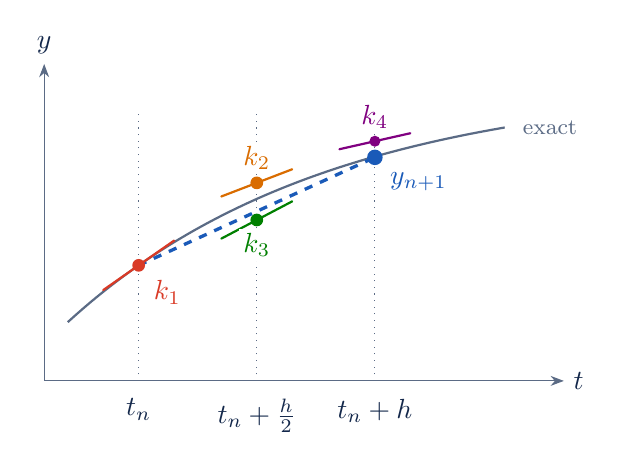
\begin{tikzpicture}[x=1.5cm,y=1.15cm,>=Stealth]
      % model: y' = 0.45(3.3-y),  exact y = 3.3 - 2.9 e^{-0.45 t}
      % the k_i below are the real RK4 slopes for one step of size h
      \pgfmathsetmacro{\tStart}{0.8}
      \pgfmathsetmacro{\hStep}{2.0}
      \pgfmathsetmacro{\tMid}{\tStart+\hStep/2}
      \pgfmathsetmacro{\tEnd}{\tStart+\hStep}
      \pgfmathsetmacro{\yStart}{3.3-2.9*exp(-0.45*\tStart)}
      \pgfmathsetmacro{\kOne}{0.45*(3.3-\yStart)}
      \pgfmathsetmacro{\yTwo}{\yStart+\hStep/2*\kOne}
      \pgfmathsetmacro{\kTwo}{0.45*(3.3-\yTwo)}
      \pgfmathsetmacro{\yThree}{\yStart+\hStep/2*\kTwo}
      \pgfmathsetmacro{\kThree}{0.45*(3.3-\yThree)}
      \pgfmathsetmacro{\yFour}{\yStart+\hStep*\kThree}
      \pgfmathsetmacro{\kFour}{0.45*(3.3-\yFour)}
      \pgfmathsetmacro{\yEnd}{\yStart+\hStep/6*(\kOne+2*\kTwo+2*\kThree+\kFour)}
      % half-length of the little slope ticks
      \pgfmathsetmacro{\dx}{0.30}
      \pgfmathsetmacro{\dyOne}{\kOne*\dx}
      \pgfmathsetmacro{\dyTwo}{\kTwo*\dx}
      \pgfmathsetmacro{\dyThree}{\kThree*\dx}
      \pgfmathsetmacro{\dyFour}{\kFour*\dx}

      \coordinate (A) at (\tStart,\yStart);
      \coordinate (B) at (\tMid,\yTwo);
      \coordinate (C) at (\tMid,\yThree);
      \coordinate (D) at (\tEnd,\yFour);
      \coordinate (F) at (\tEnd,\yEnd);

      % axes
      \draw[->,mid] (0,0) -- (4.4,0) node[right,navy] {$t$};
      \draw[->,mid] (0,0) -- (0,3.5) node[above,navy] {$y$};

      % three evaluation times
      \foreach \t in {\tStart,\tMid,\tEnd}
        \draw[dotted,mid] (\t,0) -- (\t,3.0);

      % exact solution
      \draw[thick,mid,domain=0.2:3.9,smooth,samples=60]
        plot (\x,{3.3-2.9*exp(-0.45*\x)});
      \node[mid,right=3pt,font=\footnotesize] at (3.9,{3.3-2.9*exp(-0.45*3.9)}) {exact};

      % RK4 step along the weighted slope
      \draw[very thick,rk,dashed] (A) -- (F);

      % the four slopes, drawn as short ticks
      \draw[thick,euler,line cap=round]            (A) ++(-\dx,-\dyOne)   -- ++({2*\dx},{2*\dyOne});
      \draw[thick,orange!85!black,line cap=round]  (B) ++(-\dx,-\dyTwo)   -- ++({2*\dx},{2*\dyTwo});
      \draw[thick,green!50!black,line cap=round]   (C) ++(-\dx,-\dyThree) -- ++({2*\dx},{2*\dyThree});
      \draw[thick,violet,line cap=round]           (D) ++(-\dx,-\dyFour)  -- ++({2*\dx},{2*\dyFour});

      % points
      \fill[euler] (A) circle (2.3pt);
      \fill[orange!85!black] (B) circle (2.3pt);
      \fill[green!50!black] (C) circle (2.3pt);
      \fill[violet] (D) circle (2pt);
      \fill[rk] (F) circle (2.8pt);

      % labels
      \node[euler,below right=2pt] at (A) {$k_1$};
      \node[orange!85!black,above=3pt,fill=white,inner sep=1.5pt] at (B) {$k_2$};
      \node[green!50!black,below=3pt,fill=white,inner sep=1.5pt] at (C) {$k_3$};
      \node[violet,above=3pt,fill=white,inner sep=1.5pt] at (D) {$k_4$};
      \node[rk,below right=2pt] at (F) {$y_{n+1}$};

      \node[navy,below=3pt] at (\tStart,0) {$t_n$};
      \node[navy,below=3pt] at (\tMid,0) {$t_n+\frac h2$};
      \node[navy,below=3pt] at (\tEnd,0) {$t_n+h$};
    \end{tikzpicture}
    \end{center}
    \column{0.38\textwidth}
    {\small
    \begin{align*}
      k_1&=f(t_n,y_n)\\
      k_2&=f\!\left(t_n+\tfrac h2,y_n+\tfrac h2k_1\right)\\
      k_3&=f\!\left(t_n+\tfrac h2,y_n+\tfrac h2k_2\right)\\
      k_4&=f(t_n+h,y_n+hk_3)
    \end{align*}}
    \begin{block}{Weighted average}
      \small
      \[
        y_{n+1}=y_n+\frac h6(k_1+2k_2+2k_3+k_4)
      \]
    \end{block}
  \end{columns}
\end{frame}

%% ================= 8. One step =================
\begin{frame}{One step on our model ($h=2$, $P_0=10$)}
  \vspace{-0.6ex}
  \centerline{\small $f(P)=0.5\,P\,(1-P/100)$ \qquad exact $P(2)=100/(1+9e^{-1})=23.197$}
  \vspace{0.2ex}
  \begin{columns}[T]
    \column{0.31\textwidth}
    \begin{block}{\eul{Euler}: 1 slope}
      \small\setlength{\jot}{2pt}
      $\begin{aligned}
        k_1 &= f(10)=4.500\\
        P_1 &= 10+2(4.500)\\
            &= \eul{\mathbf{19.00}}
      \end{aligned}$
    \end{block}
    \column{0.63\textwidth}
    \begin{block}{\rkc{RK4}: 4 slopes}
      \small\setlength{\jot}{2pt}
      $\begin{aligned}
        k_1 &= f(10)=4.500\\
        k_2 &= f(10+1\cdot 4.500)=f(14.50)=6.199\\
        k_3 &= f(10+1\cdot 6.199)=f(16.20)=6.787\\
        k_4 &= f(10+2\cdot 6.787)=f(23.57)=9.009\\
        P_1 &= 10+\tfrac{2}{6}\bigl(4.500+2(6.199)+2(6.787)+9.009\bigr)\\
            &= 10+\tfrac{2}{6}(39.481)=\rkc{\mathbf{23.160}}
      \end{aligned}$
    \end{block}
  \end{columns}
  \vspace{-0.4ex}
  \begin{block}{Error against the exact value}
    \centering\small
    $\eul{|19.00-23.197|=4.197}$ \qquad
    $\rkc{|23.160-23.197|=0.037}$ \qquad
    ratio $\approx \mathbf{114}$
  \end{block}
\end{frame}

%% ================= 9. MATLAB =================
\begin{frame}[fragile]{MATLAB implementation: the two update loops}
  \begin{columns}[T]
    \column{0.47\textwidth}
    \eul{\textbf{Euler}}\vspace{0.6ex}
\begin{lstlisting}[style=mat]
for i = 1:n
  y(i+1) = y(i) + ...
           h*f(t(i), y(i));
end
\end{lstlisting}
    \vspace{2ex}
    {\small Function handle keeps the solver generic:}
\begin{lstlisting}[style=mat]
f = @(t,P) r*P.*(1 - P/K);
\end{lstlisting}
    \column{0.5\textwidth}
    \rkc{\textbf{RK4}}\vspace{0.6ex}
\begin{lstlisting}[style=mat]
for i = 1:n
  k1 = f(t(i),       y(i));
  k2 = f(t(i)+h/2,   y(i)+h/2*k1);
  k3 = f(t(i)+h/2,   y(i)+h/2*k2);
  k4 = f(t(i)+h,     y(i)+h*k3);
  y(i+1) = y(i) + ...
           h/6*(k1+2*k2+2*k3+k4);
end
\end{lstlisting}
  \end{columns}
\end{frame}

%% ================= 10. Results: curves =================
\begin{frame}{Results: solution curves at a coarse step ($h=2$)}
  \begin{columns}[c]
    \column{0.64\textwidth}
    \safefig{fig_curves}
    \column{0.32\textwidth}
    \eul{Euler} drifts away from the exact curve as errors accumulate.\\[2ex]
    \rkc{RK4} stays on top of it, even with the same $h$.
  \end{columns}
\end{frame}

%% ================= 11. Error calculation =================
\begin{frame}{How we measure the error (example: $h=2$)}
  \centerline{\small $\displaystyle E(h)=\max_i\,\bigl|\,P_i-P(t_i)\,\bigr|$
    \quad over the grid $t_i=0,h,2h,\dots,20$}
  \vspace{0.6ex}
  \begin{center}
  \footnotesize
  \renewcommand{\arraystretch}{1.1}
  \setlength{\tabcolsep}{5pt}
  \begin{tabular}{@{}lcccccc@{\hspace{1.4em}}c@{}}
    \toprule
    $t$ & 0 & 2 & 4 & 6 & 8 & 10 & max over $[0,20]$\\
    \midrule
    Exact $P(t)$            & 10.00 & 23.20 & 45.09 & 69.06 & 85.85 & 94.28 & \\
    \eul{Euler} $P_i$       & 10.00 & 19.00 & 34.39 & 56.95 & 81.47 & 96.57 & \\
    \eul{Euler} $|$error$|$ & 0.00 & 4.20 & 10.70 & \eul{\textbf{12.10}} & 4.38 & 2.28 & \eul{$E=12.10$}\\
    \rkc{RK4} $P_i$         & 10.00 & 23.16 & 45.01 & 68.98 & 85.76 & 94.19 & \\
    \rkc{RK4} $|$error$|$   & 0.000 & 0.037 & 0.079 & 0.080 & 0.089 & \rkc{\textbf{0.096}} & \rkc{$E=0.096$}\\
    \bottomrule
  \end{tabular}
  \end{center}
  \vspace{-1.2ex}
  \centerline{\scriptsize\color{mid}Errors use unrounded values. For $t=12,\dots,20$ the errors are smaller, so the maxima are already found.}
  \vspace{1ex}
  \begin{block}{That gives one point on each convergence curve}
    \small
    $h=2$: \eul{Euler $E=12.10$}, \rkc{RK4 $E=0.096$}. Repeat for $h=1,\tfrac12,\tfrac14,\dots$ to trace the curves.
  \end{block}
\end{frame}

%% ================= 12. Convergence =================
\begin{frame}{Convergence: how error shrinks with step size}
  \begin{columns}[c]
    \column{0.62\textwidth}
    \safefig{fig_convergence}
    \column{0.34\textwidth}
    Slope on log-log axes equals the order.\\[1.5ex]
    \begin{block}{Halve $h$}
      \eul{Euler}: error $\div\,2$\\
      \rkc{RK4}: error $\div\,16$
    \end{block}
  \end{columns}
\end{frame}

%% ================= 13. Table =================
\begin{frame}{Measured error and reduction ratios}
  \begin{center}
  \renewcommand{\arraystretch}{1.25}
  \IfFileExists{results_table.tex}{\input{results_table.tex}}{\fbox{\parbox{\dimexpr\linewidth-2\fboxsep-2\fboxrule\relax}{\centering Run \texttt{scudem\_euler\_rk4.m} to create \texttt{\detokenize{results_table.tex}}}}}
  \end{center}
  \vspace{1ex}
  {\small\color{mid}Maximum error over $[0,20]$. Ratio is the error at the previous $h$ divided by the error at this $h$: it approaches $2$ for Euler and $16$ for RK4.}
\end{frame}

%% ================= 14. Cost =================
\begin{frame}{Is RK4 worth four slopes per step?}
  \begin{columns}[c]
    \column{0.62\textwidth}
    \safefig{fig_cost}
    \column{0.34\textwidth}
    Compared at equal \textbf{cost} (number of evaluations of $f$).\\[1.5ex]
    RK4 reaches a given accuracy with far fewer evaluations.
  \end{columns}
\end{frame}

%% ================= 15. Conclusions =================
\begin{frame}{Conclusions}
  \begin{columns}[T]
    \column{0.31\textwidth}
    \begin{block}{Euler}
      Simple, 1 slope per step, first-order accurate.
    \end{block}
    \column{0.31\textwidth}
    \begin{block}{RK4}
      4 slopes per step, fourth-order accurate. Best accuracy per unit cost here.
    \end{block}
    \column{0.31\textwidth}
    \begin{block}{Limits}
      Step size must respect stability. Stiff problems need implicit methods.
    \end{block}
  \end{columns}
  \vspace{2ex}
  \begin{center}
    \large\textbf{Choose the method to match the accuracy you need.}
  \end{center}
\end{frame}

%% ================= 16. Thanks =================
\begin{frame}[plain]
  \begin{tikzpicture}[remember picture,overlay]
    \fill[navy] (current page.south west) rectangle (current page.north east);
  \end{tikzpicture}
  \vfill
  \centering
  {\color{white}\fontsize{30}{34}\selectfont\bfseries Thank you\par}
  \vskip 1ex
  {\color{white!70!navy}\large Questions?\par}
  \vfill
\end{frame}

\end{document}
